% 第四章正文，直接编辑本文件。
\FloatBarrier\clearpage

\section{创新性说明}\label{chapter:4}

第一章将信息茧房的个人防护困难界定为``难以察觉、难以定位和难以核查''，第二章围绕这一困难给出了从浏览观测到认知体检报告的完整系统设计。本章在此基础上讨论作品的创新性。讨论遵循两个原则：其一，每项创新均对应第一章所分析的具体不足，说明现有做法为何不够、本作品改变了什么；其二，创新判断以可检验的设计差异为限，相关机制的实际作用由第三章设置的对照与消融实验分别验证，本章不作超出实验范围的效果断言。作品的四项研究任务分别对应内容内部的语义理解、内容之间的信息增量、浏览序列中的长期模式和持续分析的可信执行，本章 4.2、4.3、4.4 和 4.6 节分别讨论这四项任务的方法与系统创新，4.1 节讨论贯穿其间的问题定义创新，4.5 节讨论情绪分析的辅助方法创新，4.7 节汇总各项创新及其与现有方案的区别。

\subsection{问题定义创新}\label{section:4.1}

\subsubsection{可核查的个人浏览分析}\label{section:4.1.1}

既有研究为理解信息同质化提供了重要基础，但其分析单位与本作品面对的问题存在层次差异。传播结构研究比较平台之间用户互动的同质性\cite{ref1}，接触研究区分潜在接触、实际展示与用户点击\cite{ref3}，干预研究考察接触结构变化与态度后果的关系\cite{ref5}，国内研究则通过问卷讨论媒介使用与信息茧房指标的关联\cite{ref6}。这些工作的对象分别是群体、平台环节或自我报告，均不能回答个人层面的具体问题：某一位用户在一段时间内反复接触了什么观点，这些观点依赖哪些材料，后续内容是否补充了新的依据。

本作品的第一个创新在于把分析对象明确界定为个人授权范围内可观察、可核查的浏览经历。系统不要求掌握平台完整的社交网络，也不依赖用户事后回忆，而是以带时间索引的浏览记录为输入，将观点、论据与接触过程组织为结构化记录，并使每项结论能够回到具体片段核查。这一对象选择同时改变了结果形式：现有数字健康工具以应用时长和打开次数帮助用户发现时间分配问题\cite{ref2}，而本作品补充认知层面的解释，使同样一小时的浏览，``比较资料形成认识''与``重复接触缺少新依据的相同判断''能够被区分开来。分析的落点也由``用了多久''转向``接触了什么、依据是否增加''。

\subsubsection{以信息增量判别重复}\label{section:4.1.2}

识别同质化需要先回答``什么样的重复值得关注''。主题集中本身常对应合理的信息需求：求职期间集中研究岗位要求、升学期间集中比较院校政策，都是正常且有益的阅读。若以主题占比或观点一致性作为判别依据，持续深化的专题阅读将被误判为茧房。本作品提出以实质信息增量为核心判别线索，将其界定为新内容相对于个人此前已观察同议题历史所增加的事实、证据、限定条件、解释、反例或可执行建议，并进一步细分为事实、论据、条件、解释与行动五个维度。相同结论可以由新的数据和条件支撑，不同措辞也可能只是转述同一材料；只有同时考察观点与依据两层关系，才能区分``相同观点获得新依据''与``相同观点反复换写''。观点重复、信息增量与时间持续性三者结合，作为判别低增量同质接触的依据，补充面向个人的时长统计和单一主题分析。

\subsubsection{接触与认同的分析边界}\label{section:4.1.3}

本作品在定义阶段即明确了分析不能做什么，并将这些限制落实为系统机制而非口头声明。内容出现在屏幕上、用户可能重点阅读、用户认同其中判断，是三个不同层次，系统评估可观察接触结构，并以带置信度的行为线索估计阅读投入，不据此推断用户认同，记录中始终保留这种区分；内容中的焦虑表达与用户自身的焦虑状态分离，后者只能来自用户自愿提供的反馈；信息增量不直接代表事实真实性或个人知识增长；娱乐内容与观点型内容采用不同的解释方式，不因缺少知识增量而作负面评价。这些边界使报告始终是``用户审视自身信息环境的材料''，而不是对个人心理或认知状态的诊断。相比给出笼统风险分数的做法，将分析边界、未知比例和``证据不足''状态列为系统的正式输出，是本作品在问题定义上的具体差异。

\subsection{多模态观点理解创新}\label{section:4.2}

\subsubsection{已观察片段边界建模}\label{section:4.2.1}

现有立场检测与论证挖掘研究以完整、静态的文本为单位。SemEval-2016 立场检测任务针对给定目标的完整推文判断立场\cite{ref8}，IAM 在完整文档上联合抽取主张、立场与论据\cite{ref13}，T-MAD 等多模态立场方法假设相关模态均已获得\cite{ref14}。真实浏览场景不满足这些假设：用户可能只看视频开头数秒，画面文字可能属于受访者而非作者，观点可能在后续口播中被反驳，各模态还可能分别缺失。将不完整片段按完整内容处理，正是混同讨论对象、发言主体与实际立场的根源。

本作品提出已观察多模态前缀的建模方式（定义 2-1，式 2-1、2-2），按片段首次被观察到的时间组织模型输入，使分析范围始终等于用户实际接触的范围，未被观察的内容不进入接触记录。在此基础上，论证单元统一记录讨论对象、表达主体、主张、论据、适用条件、单元间关系及证据索引，正文与评论分别建立单元并保留父项关系。由此，``用户看到了什么''成为模型的形式化输入条件，后续的历史比较与时序分析均建立在这一范围之上。

\subsubsection{目标对齐与质量门控}\label{section:4.2.2}

跨模态理解的常见做法是拼接各模态表示后统一分类，模态冲突在这种结构中容易被掩盖。本作品采用目标条件的跨模态对齐：围绕当前讨论对象分别查询文字、画面与音频词元，对齐过程加入媒体时间距离与画面空间关系偏置（式 2-3 至 2-5），再以对象相关性、识别质量、画面清晰度与片段覆盖状态为输入进行质量门控（式 2-6 至 2-8）。对象条件决定``应关注哪些片段''，质量门控决定``这些片段各占多大比重''，二者分工明确。当字幕与口播真实存在分歧时，系统输出两者的表达内容及冲突关系，而非强行融合为单一立场；观点归属、证据定位与充分度估计由联合损失共同训练（式 2-15 至 2-19），各自保留中间结果以支持逐项消融检验。对真实分歧的保留和对各机制贡献的可分离评价，是本方法相对于端到端融合方案的两点具体改进。

\subsubsection{可修订理解与双层证据}\label{section:4.2.3}

连续浏览中，理解结果必须能够随新片段到达而更新。本作品为每个字段独立估计证据充分度，区分``可输出''与``证据待补充''两种状态（式 2-13、2-14），使模型可以先呈现已确定的主张、暂缓不确定的归属，待补充片段到达后按版本修订。增量更新以受影响的对象和论证单元为范围，字段级差异向后传递至历史比较与图谱模块，旧版本保留用于追溯。与之配合的是论据与证据索引的双层记录：论据是原文用于支持判断的材料，证据索引是系统抽取该字段所依据的原文位置，两层关系分别保存。前者使历史比较能够检查材料层面的重复，后者使用户能够核查模型判断的出处。按此设计，每一项语义判断都附带出处，每一次修订都保留轨迹；可解释性不再是事后附加的展示功能，而是输出结构本身的约束。

\subsection{个人历史比较创新}\label{section:4.3}

\subsubsection{观点与论据双路表示}\label{section:4.3.1}

判断内容是否重复，通常依赖主题标签或整体文本相似度，这类方法无法区分两种关键情形：结论相同但提供了新数据、新条件的材料，与措辞迥异却只是复述同一来源的材料。本作品将重复判定分解为观点与论据两条通路（式 2-22、2-23）：观点分支回答``是否对同一对象作出相近判断''，论据分支回答``支撑材料、条件与解释是否重合''。两条通路的对比学习目标相反相成（式 2-24）——观点分支将相近判断拉近，论据分支却把``同一结论下的新数据、新事实''推远，使``同观点、新论据''这一最易混淆的情形在两路获得方向相反的学习信号。训练样本专门覆盖同观点新依据、同依据换措辞、不同作者引用同一材料及引用后反驳等难例，并以时间、否定和群体条件仅有少数字词差异的样本强化条件识别。训练目标围绕这些易混淆情形组织，这是双路表示区别于通用语义匹配的关键。

\subsubsection{条件约束与联合覆盖}\label{section:4.3.2}

增量比较的前提是两份材料可以比较。本作品将对象、时间范围、地区与人群等适用条件作为比较的先决约束：``当前招聘形势较差''与``未来需求可能恢复''分属现状与预期，``某地区应届生''与``整体就业市场''适用范围不同，均不能仅因措辞相近而判为重复。可比范围被显式标注为``相同范围''\,``扩展条件''与``范围待定''，条件扩展本身作为增量的一种类型进入统计，而非被相似度计算吸收。

单条历史材料往往只覆盖当前内容的一部分。本作品的联合覆盖模型读取当前信息单元与多条历史证据的并集（式 2-26、2-27），能够识别``每条旧材料各覆盖一部分、合起来已覆盖全部''的情形，避免仅因没有单一来源完整重合就误判为新增。覆盖判断同时返回实际使用的历史片段标识，使检索遗漏与覆盖误判可以在评价中被分开定位。增量输出不是单一新颖度分数，而是事实、论据、条件、解释与行动五个维度的新增比例及各自的待定比例（式 2-28 至 2-30），``新案例持续出现、讨论范围长期不变''这类结构性重复因此在向量层面保留了可区分的特征。低增量得分综合五维增量、覆盖比例与条件关系后经独立校准（式 2-32、2-33），作为时序分析的输入。由此形成的增量刻画分维呈现、分母明确并保留待定状态，比单一相似度分数更细致地区分了重复的类型。

\subsection{长期接触模式识别创新}\label{section:4.4}

\subsubsection{语义与观察分层时序图}\label{section:4.4.1}

将分析单位从内容之间的关系扩展到个人在一段时间内的接触过程，需要一种同时保存论证结构与接触证据的表示。本作品构建的个人时序论证图（定义 2-3）包含内容、观点、论据、来源四类节点和表达、支持、反驳、限定、引用、复述六类关系，每条语义边均连接原文依据、置信信息与生效版本。图的两个层次分别维护：语义层回答``哪些内容表达或支持相近判断''，观察层回答``用户接触了其中哪些片段、投入多少时间''。同一论据被多个作者引用时通过来源关系连接到共享材料，使``发布者众多''与``材料源头单一''可以同时成立、分别呈现；同一内容被重复浏览时复用已有语义节点、新增观察事件，内容重复与接触次数增加由此得到区分。图的建立完全基于个人授权范围内的浏览记录，无须平台社交网络数据，这使群体层面研究方法\cite{ref1,ref3}所依赖的数据条件不再是个人层面分析的前提。

\subsubsection{统计与记忆双路读出}\label{section:4.4.2}

本作品的识别模型由可解释图统计与时序图学习两路组成，两路共享同一张图、读取同一份事件记录。可解释一路计算观点集中度、低增量接触占比、旧论据复用程度、持续比例与最长连续长度（式 2-38 至 2-46），每个指标的分母、有效权重与未知比例均随结果保存；时序一路借鉴 Temporal Graph Networks 的事件消息与节点记忆机制\cite{ref16}，将阅读权重、表达方向、增量向量、来源状态与缺失掩码共同写入消息（式 2-47 至 2-49），学习反复接触的顺序与间隔，窗口读出时两路特征共同进入分类（式 2-50 至 2-52）。这一结构的设计意图是使两条路线互为检验：消融实验可以分别去除阅读权重、论据边、来源关系或时间特征，考察各部分对识别质量与误报的实际贡献；面向用户的解释不由模型记忆生成，而由图中的实际关系与可重算统计生成，用户可以从任何一项长期结论回溯到具体日期、具体观点和具体材料。两路之中，学习模型负责发现序列模式，可解释统计负责约束结论的证据形式。

\subsubsection{覆盖门控与对照约束}\label{section:4.4.3}

长期结论的可信程度取决于观察基础。本作品为每个窗口计算语义覆盖率（式 2-43），将采集缺口、未归属时间与待分析份额保留在统计之中，覆盖不达标的窗口直接输出``证据不足''而非低置信的猜测；持续性只按有效观察日计算，无采集记录的日期中断连续段。模型训练中，持续查阅考试政策、围绕一个行业比较岗位、阅读结论一致但数据独立的材料、情绪强烈但具有新依据的内容，均作为正常专题阅读的负类对照，使``观点集中''与``低增量重复''在监督信号层面被迫分离。这些机制共同保证：系统对用户给出的每一个长期判断，都能同时说明其证据范围和证据缺口。

\subsection{情绪与处境分析创新}\label{section:4.5}

情绪分析在本作品中不是独立的情感分类任务，而是理解低增量重复的一条辅助维度，其创新体现在三个方面。

其一，情绪被组织为带证据的结构化框架（定义 2-5）。现有情绪---诱因研究以完整文本中的配对抽取为主\cite{ref23,ref24}，本作品将框架扩展为情绪、诱因、持有者、指向对象、认知评价、生活处境、表达方式与归属关系的联合表示，每个字段均保存原文与时间索引。发布者、语者与情绪持有者分别记录：作者转述求职者的担忧时，情绪归于被描述的求职者；引用被后文否定时，被引述的担忧与作者的反驳分别保存。这使报告能够区分``用户接触了焦虑表达''与``用户接触了反驳焦虑的内容''。

其二，内容如何呈现处境被显式建模。认知评价选取目标受阻、威胁或损失、结果不确定性、自身控制可能与应对资源五个维度，以有序阈值估计强度（式 2-84 至 2-87），并将``未提及''与具体评分分离处理\cite{ref27}；灾难化概括、社会比较与紧迫性施压作为表达方式单独标注，各自对应可定位的措辞证据；生活处境采用层级标签并以条件化方式联合预测（式 2-91、2-92），使``求职流程说明''与``担心求职失败''形成不同输出。由此，系统描述的不是笼统的正负面情绪，而是``围绕什么处境、以什么方式、由谁表达的担忧''。

其三，内容情绪与个人感受在数据流层面彻底分离。内容框架描述的是材料中的人物与表达；用户真实感受的标签来自其自愿提供的自报反馈，个体校准结果单独标注为估计。个体校准在内容模型固定的前提下只更新个人偏置（式 2-95、2-96），且更新过程限定在可信执行环境内，共享参数的改进使用另行授权的研究数据。这一设计把``避免将信息判断误写为心理诊断''的原则落实为可检查的工程边界。

\subsection{隐私保护与持续分析创新}\label{section:4.6}

\subsubsection{贯穿全程的机密计算协议}\label{section:4.6.1}

浏览记录反映个人现实处境，隐私保护是本作品能够被放心使用的前提，而非附加功能。现有机密计算实践多解决单次推理或存储的隔离问题\cite{ref10,ref22}，本作品将其扩展为贯穿数据接收、模型执行、历史更新与结果返回的完整协议，创新点有三。第一，证明对象从执行环境扩展到分析配置：受证明加载器核验模型权重、提示模板与分析配置的摘要，形成版本清单并与会话挑战、通信端点共同绑定到硬件证明（式 2-55 至 2-57），密钥按用途与方向分离派生（式 2-58、2-59），使用户能够确认数据交给了获准运行的那一版程序，版本切换必须重新建立绑定。第二，保护对象从原始内容扩展到全部派生数据：语义向量、观点图、分析报告与原始片段纳入同一可信边界与同一管理流程，涉及 GPU 推理时设备、明文传输与计算一并处于受证明范围内\cite{ref17}，避免``只保护输入、遗漏中间结果''的常见缺口。第三，历史状态的新鲜度与可删除性获得协议级保障：客户端保存的检查点构成防回退锚点（定义 2-4，式 2-62、2-63），宿主机提供旧快照即可被识别；用户删除记录时，受影响状态按时序依赖闭包从有效检查点重放重建（式 2-64、2-65），向量、图关系与统计结果随原始记录同步更新。上述三点将远程证明、长期状态管理与派生数据删除整合为一套面向连续认知分析的协议，覆盖了现有实践中常被遗漏的配置一致性与派生数据环节。

\subsubsection{基于版本的异步修订}\label{section:4.6.2}

持续浏览要求分析与用户的快速切换并行，安全机制又不能破坏结果的正确归属。本作品的异步设计以事件标识、输入片段版本与模型版本三元组为枢纽：每次分析结果绑定其对应的浏览事件和输入版本，用户划走后迟到的结果仍写回原事件，新增片段引发的修订通过撤销旧版本统计贡献、应用新版本的方式传播，手机快速切换、服务器异步处理与用户事后更正进入同一条可追溯的更新流程。内容对象、接触事件与语义结果三层记录相互引用，同一视频的新字幕补充到原内容对象，再次打开同一帖子产生新接触事件，既支持重复接触统计，也保留材料唯一性。由此，第二章各算法模块的修订能力（2.4 至 2.6 节）与安全协议的版本管理（2.7 节）在系统层面闭合，作品得以作为持续运行的工具存在，而非一次性的分析脚本。

\subsection{创新点总览}\label{section:4.7}

图~\ref{fig:4-1} 汇总六项创新与应用目标、共同主线之间的关系。

\begin{figure}[htbp]
\centering
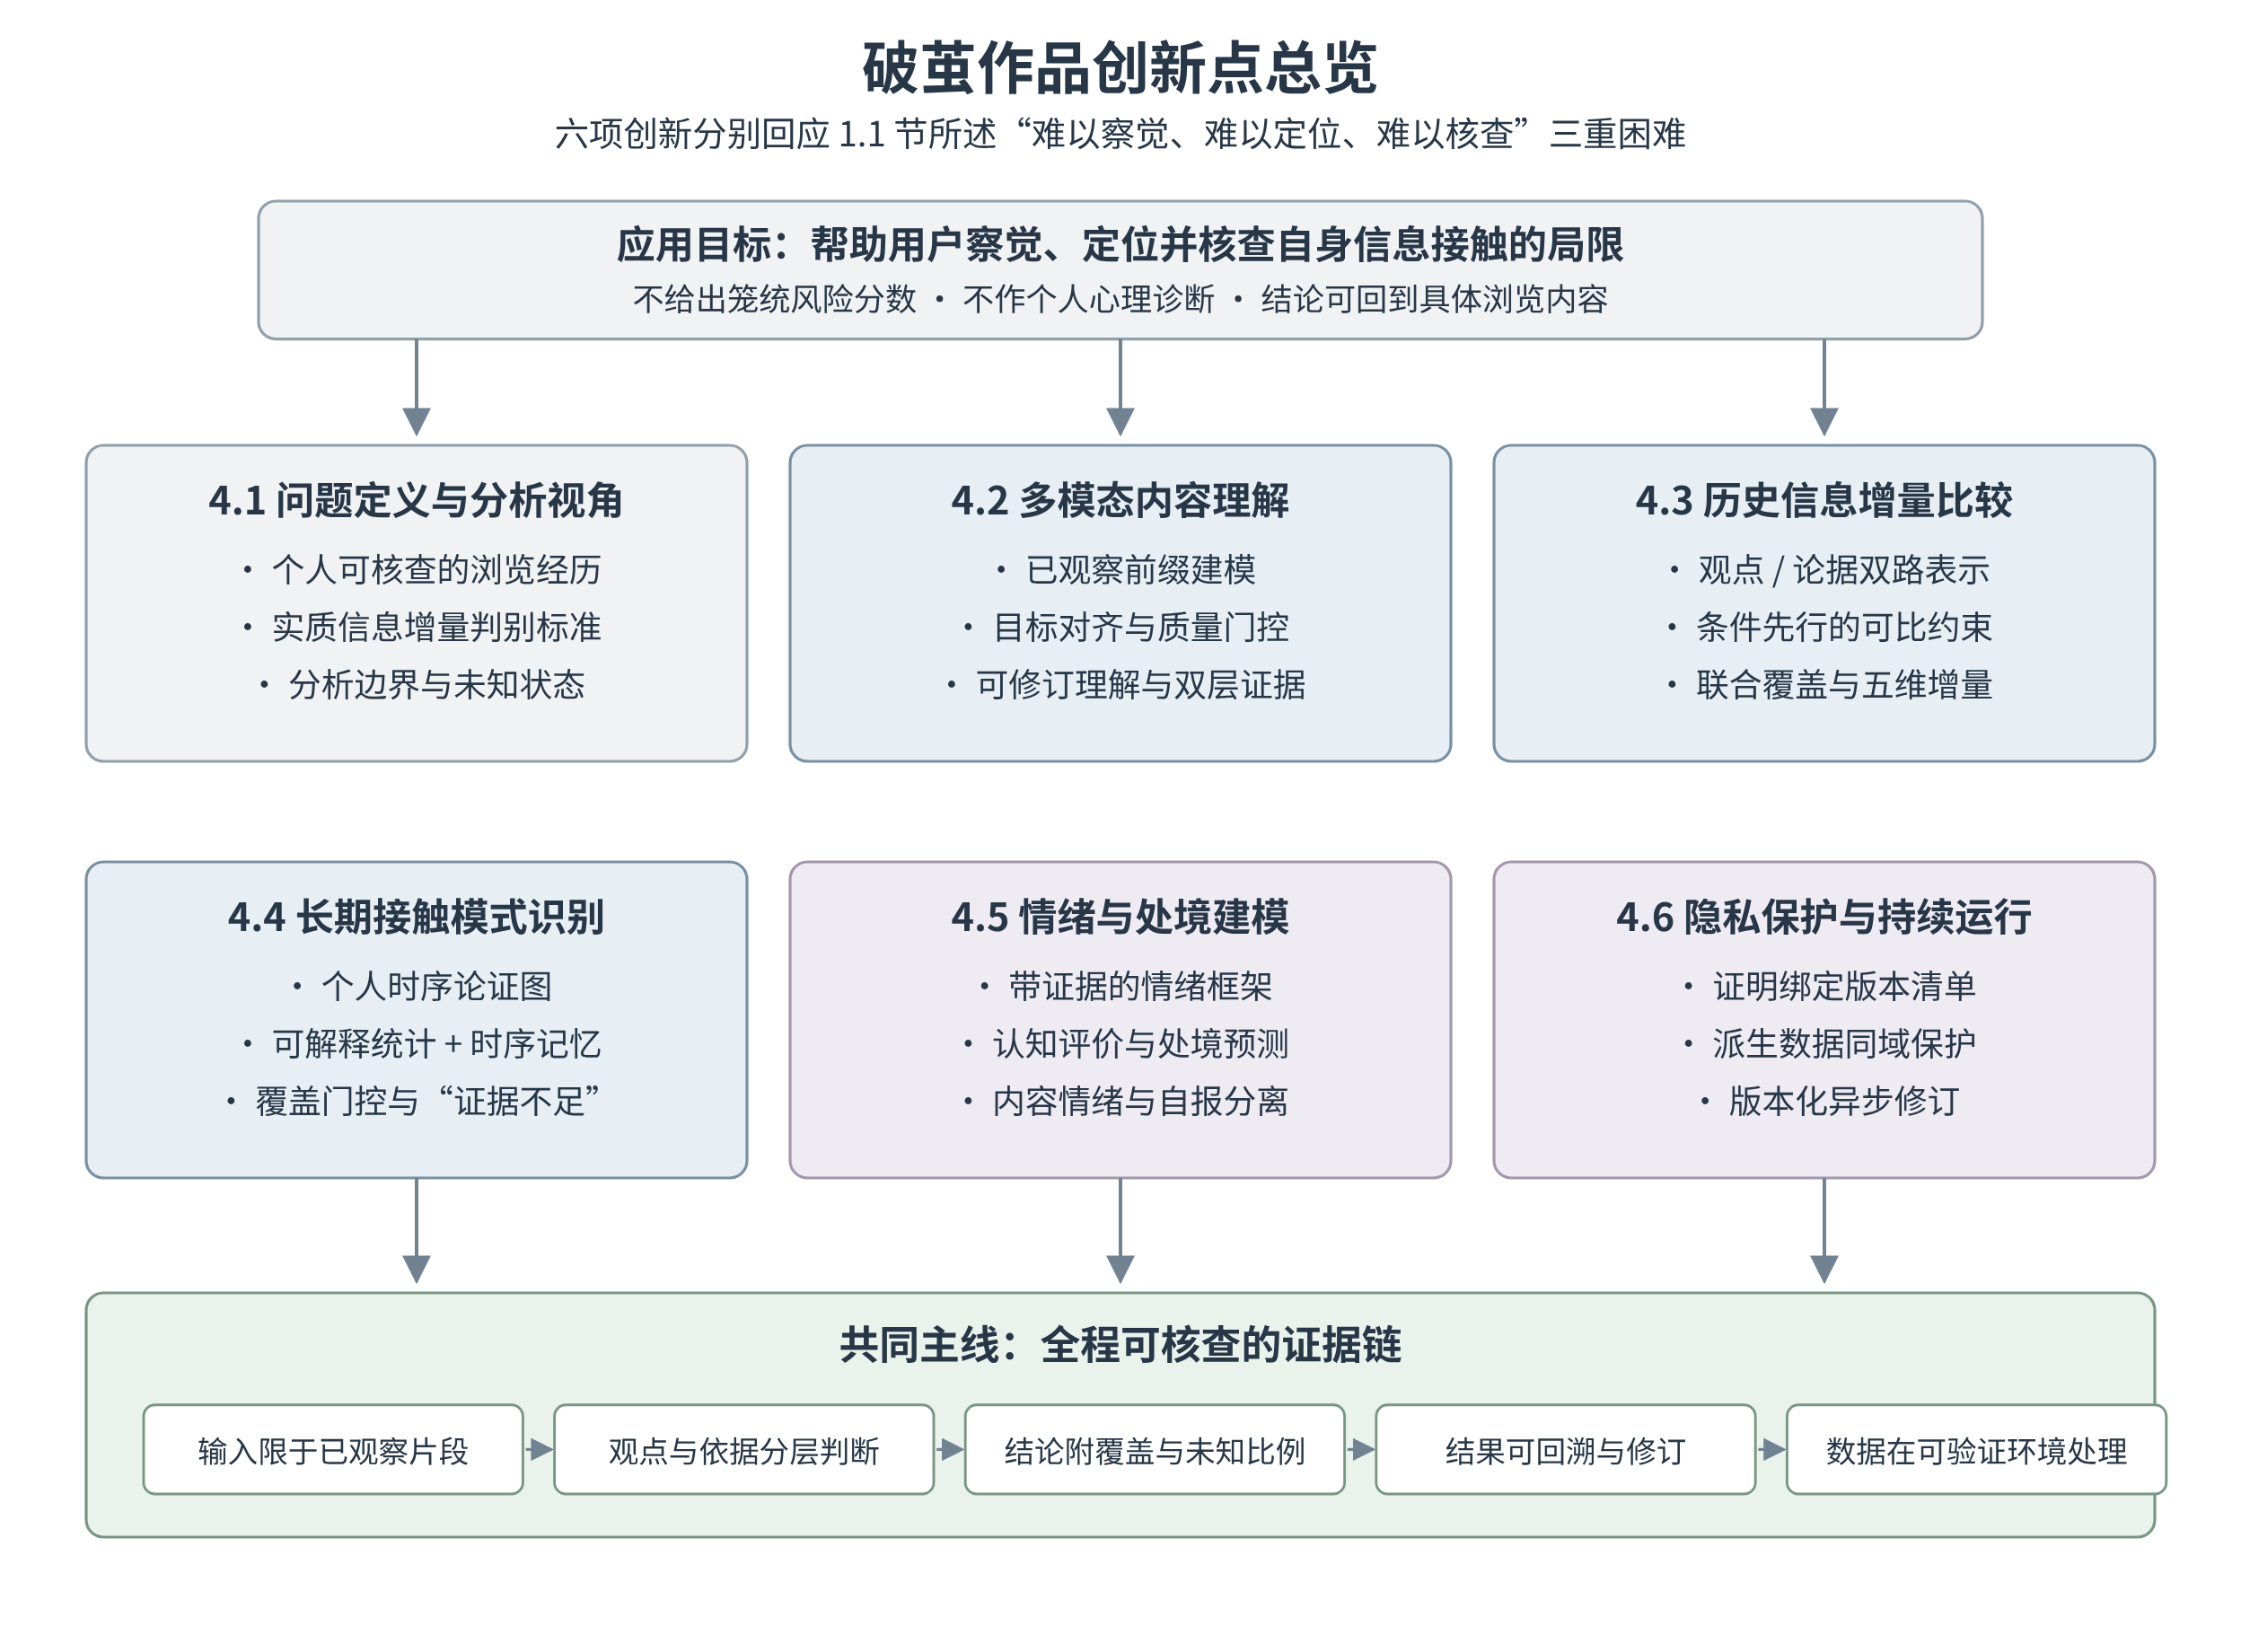
\includegraphics[width=\linewidth,height=0.66\textheight,keepaspectratio]{figures/chapter4/fig_4_1_innovation_overview.png}
\caption{破茧作品创新点总览}\label{fig:4-1}
\end{figure}

六项创新分别回应``难以察觉、难以定位、难以核查''三重困难，并以全程可核查的证据链为共同主线。

表~\ref{tab:4-1} 将上述创新按``现有方案的典型做法---本作品的做法---创新指向的问题''汇总。各项创新分别对应第三章设置的实验对照：内容理解层比较纯文本、模态拼接与完整证据约束方法，并消融对象条件、质量门控与证据监督，部分观察阶段的比较用于评价后续片段到达时的修订效果；历史比较层检验双路表示对``同观点新依据''与``换写旧材料''的区分能力；长期识别层通过去除历史增量、来源关系、时间编码与记忆考察各要素贡献；机密计算层测量证明、传输、推理与提交各阶段的开销及安全用例的实际拦截环节。创新的成立以这些对照结果为依据，不以功能存在本身为据。

\begin{longtable}[]{@{}
  >{\RaggedRight\arraybackslash}p{(\linewidth - 6\tabcolsep) * \real{0.2500}}
  >{\RaggedRight\arraybackslash}p{(\linewidth - 6\tabcolsep) * \real{0.2500}}
  >{\RaggedRight\arraybackslash}p{(\linewidth - 6\tabcolsep) * \real{0.2500}}
  >{\RaggedRight\arraybackslash}p{(\linewidth - 6\tabcolsep) * \real{0.2500}}@{}}
\caption{本作品与现有方案的主要区别}\label{tab:4-1}\tabularnewline
\toprule\noalign{}
层面 & 现有方案的典型做法 & 本作品的做法 & 创新指向的问题 \\
\midrule\noalign{}
\endfirsthead
\toprule\noalign{}
层面 & 现有方案的典型做法 & 本作品的做法 & 创新指向的问题 \\
\midrule\noalign{}
\endhead
\bottomrule\noalign{}
\endlastfoot
分析对象 & 群体传播结构、平台环节或问卷自报\cite{ref1,ref3,ref6}；数字健康工具统计时长\cite{ref2} & 个人授权范围内可核查的浏览经历，结论可回到具体片段 & 茧房难以被个人察觉、定位与核查 \\
判别标准 & 主题占比、观点一致性或文本相似度 & 观点重复、五维实质信息增量与时间持续性三者结合 & 误伤合理的专题阅读，漏判换写式重复 \\
内容理解 & 完整文本的立场或论证抽取\cite{ref8,ref13}，模态齐全的多模态融合\cite{ref14} & 已观察前缀建模、目标条件对齐、质量门控、可修订理解与双层证据记录 & 局部、冲突、快速变化的实际浏览输入 \\
历史比较 & 单一文本相似度或整体语义匹配 & 观点与论据双路表示、条件先行约束、多历史联合覆盖 & 同观点新依据与换写旧材料的混淆 \\
长期评估 & 静态快照、时长统计或黑箱模型评分 & 个人时序论证图，可解释统计与时序记忆双路读出，覆盖门控输出``证据不足'' & 长期模式的识别与可解释兼得 \\
情绪分析 & 笼统正负面分类，或将内容情绪等同用户感受 & 带证据的情绪框架、认知评价与处境联合建模，内容情绪与自报反馈数据流分离 & 焦虑表达的情境化理解与心理诊断误写 \\
隐私保护 & 服务端明文处理，或仅本地简单统计 & 证明绑定版本清单、派生数据同域保护、检查点防回退、删除依赖重放 & 持续认知分析中的明文暴露与状态篡改 \\
持续运行 & 一次性分析或简单缓存 & 事件---输入---模型版本三元组驱动的异步修订与统计更新 & 快速浏览现实与分析正确归属的矛盾 \\
\end{longtable}

\subsection{本章小结}\label{section:4.8}

本章从问题定义、内容理解、历史比较、长期识别、情绪建模、隐私保护与持续运行七个层面说明了作品的创新性。贯穿其中的共同线索是：本作品不追求给出一个更灵敏的茧房分数，而是把分析建立为一条用户可以全程核查的证据链——输入限定于实际观察的片段，判断区分观点与依据两层关系，长期结论附带覆盖与未知状态，结果可以回到原文修订，个人数据在可验证的环境中处理。各项创新分别对应第三章的对照与消融实验，其实际改进幅度以实验结果为准；对用户认知觉察的最终帮助，则留待用户研究检验。
